
\graphicspath{ {mainmatter/Wright_2003/} }

\label{chapter:Wright_2003}
\title*{2003: OpenSound Control: State of the Art 2003}
\titlerunning{OpenSound Control}

\author{Matthew Wright, Adrian Freed and Ali Momeni}
\authorrunning{Wright et al.}


% \institute{Matthew Wright \at Center for New Music and Audio Technology (CNMAT), Univ. California, Berkeley, 1750 Arch St., Berkeley, CA  94709, \email{matt@cnmat.berkeley.edu}
% \and Adrian Freed \at CNMAT, Univ. California, Berkeley, 1750 Arch St., Berkeley, CA  94709, \email{adrian@cnmat.berkeley.edu}
% \and Ali Momeni \at CNMAT, Univ. California, Berkeley, 1750 Arch St., Berkeley, CA  94709, \email{ali@cnmat.berkeley.edu}}
%
%
\maketitle

\abstract*{OpenSound Control (``OSC'') is a protocol for communication among computers, sound synthesizers, and other multimedia devices that is optimized for modern networking technology.  OSC has achieved wide use in the field of computer-based new interfaces for musical expression for wide-area and local-area networked distributed music systems, inter-process communication, and even within a single application.}


\section{Tutorial Overview of OSC}

This is a user-level overview of OSC.  For more technical details such as exact
semantics and the binary format of OSC messages, please see the OSC specification
 \cite{Wright:2002}.

\subsection{Client/Server}

OSC is designed to support a client/server architecture.  OSC data is
transmitted in data units called \textit{packets}.  Anything that sends OSC
packets (e.g., an application, physical device, subprogram, etc.) is a
\textit{client} and anything that receives OSC packets is a \textit{server}.

OSC is a transport-independent, high-level application protocol; in other words,
OSC does not specify what low-level networking mechanism will be used to move OSC
packets from the client to the server.

\subsection{Messages}

The basic unit of OSC data is a \textit{message}, consisting of an
\textit{address pattern,} a \textit{type tag string,} and \textit{arguments}. 
The address pattern is a string that specifies the entity or entities within the
OSC server to which the message is directed (within the ``Addressing Scheme''
described below) as well as what kind of message it is. The type tag string gives
the data type of each argument.  The arguments are the data contained in the
message.

For example, a message's address pattern might be /voice/3/freq, its type string
might indicate that there is a single floating-point argument, and the argument
might be 261.62558.

\subsection{Argument Data Types}

Each message contains a sequence of zero or more arguments. The official OSC
data types are ASCII strings, 32-bit floating point and integer numbers, and
``blobs,'' chunks of arbitrary binary data. OSC's type mechanism allows for many
other types, including 64-bit numbers, RGBA color, ``True,'' and ``False.''  Only
a few implementations support these other types, but they all represent them in a
standard way.


\subsection{Addressing Scheme}

All of the points of control of an OSC server are organized into a
tree-structured hierarchy called the server's \textit{address space}. Each node
of the address space has a symbolic name and is a potential destination for OSC
messages.

Each OSC server defines its own address space according to the features it
provides and the implementor's idea of how these features should be organized. 
This is in contrast to protocols such as ZIPI \cite{McMillen:1994} and MIDI that attempt to
define in advance what the architecture of a synthesizer should be and what kinds
of messages can be sent to it.

An OSC \textit{address} is simply the full path from the root of the address
space tree to a particular node, with a slash-delimited format like a URL or file
system pathname. For example, the address \texttt{/voices/3/freq} refers to a node
named ``freq'' that is a child of a node named ``3'' that is a child of a
top-level node named ``voices.''

An OSC server's address space may change dynamically, therefore OSC's query
system (described below) includes a mechanism for discovering the current address
space.

\subsection{Address Pattern Matching}

Remember that each OSC message contains an OSC address \textit{pattern}, not an
OSC address.  An OSC address pattern is exactly like an OSC address, except that
it may contain special characters for regular expression \cite{Friedl:1997} pattern matching. 
When an message's address pattern matches more than one of the addresses in the
server's address space, the effect is the same as if there were individual
messages (all with the same arguments) sent to each of the matched addresses.

The special characters are `?,' `*,' a string of characters inside `[brackets],'
and a comma-delimited list of strings inside `\{curly,braces\}.'  They work like
Unix shell filename globbing.

\subsection{Bundles and Temporal Atomicity}

A \textit{bundle} is a sequence of messages and/or bundles.  This recursive
definition allows for arbitrary nesting of sub-bundles.  All of the messages in
the same bundle must be processed by the OSC server atomically; in other words it
should be as if all of the messages in the bundle are processed in a single
instant.  An OSC packet may be a bundle or a (single) message.

\subsection{Time Tags}

Each bundle has a \textit{time tag }that specifies the desired absolute time at
which the messages in the bundle should take effect.  The format is that used by
the Internet Network Time Protocol \cite{Mills:1992} and provides sub-nanosecond accuracy over
a range of over 100 years.  OSC currently relies on an outside mechanism to
synchronize clocks on different machines to the same absolute time, for example,
NTP \cite{Mills:1992} or SNTP \cite{Mills:1996}.

\subsection{Queries}

\textit{Queries} are OSC messages that request the server to send information
back to the client. Example queries include ``what is the current list of nodes
under this given node?,'' ``what argument types are expected for messages sent to
this given node?,'' ``what is the value of the parameter that can be set by
sending messages to this node?,'' and ``please send me some documentation for the
object or feature specified by this address.''

\section{Implementations of OSC }

CNMAT created OSC and maintains a web site, downloadable code, and developers'
email list.  As the public face of OSC we often hear about other people's use of
OSC; this section lists the implementations and uses of OSC of which we are
aware.  Since the standard is open and our code is freely downloadable, we assume
that there are other implementations of which we are not aware; we look forward
to hearing about them.  No doubt some of the details described in this section
will be obsolete by the time this paper goes to press, especially, we hope, some
of the limitations of certain systems.

All of the implementations mentioned in this section are linked from the main
OSC home page at CNMAT.\footnote{\url{http://www.cnmat.berkeley.edu/OSC}}

\subsection{CNMAT's Open-Source OSC Software}

%All of the software mentioned in this section is available for download from CNMAT (http://www.cnmat.berkeley.edu/OSC).

When we introduced OSC in 1997, we released \textit{OSC-client.c}, a C library
for constructing OSC packets through a procedure call interface. There is nothing
more to implementing an OSC client than constructing proper OSC packets and
sending them over the network.

We also released a pair of text-based Unix command-line utilities:
\textit{sendOSC} allows the user to type in message addresses and arguments via a
no-frills text interface, and formats and sends these messages via UDP to the
desired IP address and port number; \textit{dumpOSC} listens for OSC messages on
a given UDP port and prints them out in a simple ASCII format.

As part of CNMAT's early efforts to promote OSC, we released the \textit{OSC
Kit} \cite{Wright:1998a} in source code form in 1998.  Our reasoning was that although the
community as a whole was in favor of OSC and its features (as they had been of
ZIPI), people would be reluctant to implement OSC (as they had been of ZIPI)
unless we did a lot of the work for them (which we did not do for ZIPI). Thus,
the OSC Kit implements most of the features needed for an OSC server: (dynamic)
construction of an address space,  parsing OSC packets, pattern-matching address
patterns within the address space, associating a user-defined callback procedure
with each node of the address space and invoking that procedure in response to
messages sent to that node, and even a scheduler for implementing time tags.  The
OSC Kit is completely neutral to architecture and operating system and was
designed not to degrade reactive real-time performance.

\subsection{Music Programming Environments}

All of the current OSC implementations known to the authors send and receive OSC
packets only as UDP packets.

\subsubsection{Max/MSP}

The first programming environment to implement OSC was \textit{Max/MSP} \cite{Puckette:1991,Zicarelli:1998}, in the form of Max ``externals'' written by Matt Wright. The
\textit{OpenSoundControl} external translates in both directions between native
Max data lists and OSC-formatted binary data.  The \textit{otudp} external (as
well as the now-obsolete \textit{udp} external) sends and receives arbitrary UDP
packets and can be used in conjunction with the \textit{OpenSoundControl} object.
 These are implemented as separate objects to allow for transmission of OSC
packets other than by UDP packets and to allow for transmission of UDP packets
other than OSC packets.  Finally, the \textit{OSC-route} external enables the
parsing of OSC address patterns by Max programmers and implements OSC's pattern
matching features. All of these objects have been ported to the OSX version of
Max/MSP.

The Max/MSP implementation has full support for sending and receiving messages
and bundles, but there is currently no integration between OSC time tags and
Max's scheduler and no support for queries.  There is backwards-compatible
support for both sending and receiving non-type-tagged messages.  Temporal
atomicity of bundles is handled by the fact that \textit{OpenSoundControl}
outputs a ``bang'' after outputting all of the messages in a bundle; it is the
responsibility of the Max/MSP programmer to ensure that all of the messages take
effect atomically when the ``bang'' is output.

\subsubsection{SuperCollider}

James McCartney added OSC support to the object-oriented \textit{SuperCollider}
(``SC'') language and environment \cite{McCartney:2000} in 1998.  The \textit{OSCNode} object
represents a node of the OSC address space and contains a symbolic name, a list
of the children of the node, and a function to be called when the node receives a
message. The \textit{OSCOutPort} and \textit{OSCInPort} objects represent UDP
ports that can send or receive (respectively) OSC packets.  Every
\textit{OSCInPort} has an \textit{OSCNode} that is the root of the address space
associated with that port.

There is a large sub-tree of OSC messages that can be sent to the SC environment
itself, including ``run the main patch,'' ``stop synthesis,'' ``play this sound
file from the local disk,'' and even ``compile and execute the code in the string
argument to this message.''  There is also an OSC representation for all of the
important MIDI messages (note on/off, continuous controllers, pitch bend, program
change, channel and key pressure,  and all-notes-off); when SC receives one of
these OSC messages it's exactly as if SC had received the corresponding MIDI
message via MIDI input.

Version 3 of SC, only for OSX, has a completely new architecture and is called
\textit{SuperCollider Server}.  In this version, the synthesis engine is a
separate application from the SC language and programming environment; the two
communicate exclusively with OSC messages via UDP or TCP.  This allows the SC
synthesis engine to be controlled by applications other than the SC language.

\subsubsection{Open Sound World}

\textit{Open Sound World} (OSW) \cite{Chaudhary:1999} is a scalable, extensible object-oriented
language that allows sound designers and musicians to process sound in response
to expressive real-time control.  OSW has the same graphical dataflow model and
nested subpatch structure as the Max family of languages; one important
difference is that every OSW object has a symbolic name.  Thus, the objects in an
OSW patch automatically form an OSC-style hierarchical address space and can thus
easily be addressed with OSC messages; the OSW kernel handles this automatically.
 OSW also provides an object called \textit{OSCListen} that can be used to
process incoming OSC messages manually; this allows OSW programmers to construct
an OSC address space that does not necessarily reflect the tree structure of the
OSW program that is the OSC server.

OSW has the best support of OSC queries of any implementation known to the
authors, thanks in large part to recent work by Andy Schmeder at CNMAT.  The
dynamic address space of an OSW program can be discovered by a querying client.
Any message that can be understood by any of the objects in an OSW patch can be
sent to that object via OSC.  An OSC client can get the current value of any
variable of any OSW object.

OSW fully supports type tags.  There is currently no connection between OSC time
tags and OSW's notion of the current time.  A careful programmer can use OSW's
``synchronous outlets'' mechanism to ensure that all elements within a bundle
will be processed atomically.

\subsubsection{Pd}

OSC support in the \textit{Pd} programming language and environment \cite{Puckette:1996} is in
the form of third-party objects.  The \textit{sendOSC} and \textit{dumpOSC}
objects are for sending and receiving OSC packets and are derived from CNMAT's
text-based Unix command-line utilities of the same name.

The \textit{sendOSC} object must be set to write to a given IP address and UDP
port.  Then it translates Pd lists to properly-formatted OSC messages and sends
them.  There is also support for creating bundles, but not for specifying
bundles' time tags.

The \textit{dumpOSC} object creates a UDP socket, parses incoming OSC packets on
that port, converts each OSC message to a Pd list, and outputs the lists
sequentially.  Time tags are ignored.  There is no mechanism to assist with
temporal atomicity of bundles; in fact, no representation of the bundle structure
of incoming OSC packets is available to the Pd programmer---consecutive lists
output by \textit{dumpOSC} might be from the same bundle or from different OSC
packets entirely.

The \textit{routeOSC} object is derived from and practically identical to the
Max/MSP \textit{OSC-route} object; it supports the parsing of address patterns
with pattern matching.

Pd does not currently support queries.

\subsubsection{Virtual Sound Server}

NCSA's \textit{Virtual Sound Server} (``VSS'') \cite{Bargar:1994} is an environment for
real-time interactive sound synthesis; it is designed to be used in conjunction
with graphics rendering software and includes mechanisms for synchronization of
its audio with other applications' video.  VSS can be controlled with a limited
form of OSC utilizing a flat address space.  Type tag strings, pattern matching,
bundles, time tags and queries are not supported.

\subsubsection{Csound}

Csound support for OSC currently exists only as part of the ``unofficial''
release.\footnote{\url{http://web.tiscali.it/mupuxeddu/csound}}  This implementation is based
on the OSC Kit and allows users to define Csound orchestras that can be
controlled by OSC. The Csound programmer can name elements of the OSC address
space, but the overall tree structure of the OSC address space is constrained by
the fact that all Csound instruments are at the same level in a flat namespace. 
A procedure called at the K-rate checks for  and processes newly-received OSC
messages.

\subsection{Software Synthesizers}

\textit{Grainwave} \cite{Berry:2002} is a software granular synthesizer with very limited OSC
support. It accepts MIDI messages formatted as OSC messages; the use of OSC is
solely as a mechanism to transmit MIDI-style data over the Internet.

Native Instruments' \textit{Reaktor}\footnote{\url{http://www.native-instruments.com}} is a
general-purpose environment for building software synthesizers. Reaktor's OSC
support in version 3 is similar to Grainwave's, essentially just MIDI over the
Internet, but version 4, currently still in beta, is said to have much more
integrated OSC support.

\subsection{General Purpose Programming Languages}

All of the implementations described in this section are available in source code form via CNMAT's OSC home page.

Chandrasekhar Ramakrishnan has implemented Java classes that can create OSC packets via a procedural interface and send them in UDP packets \cite{Ramakrishnan:2003}.  It supports type tags but not time tags.  Future plans include the ability to
receive OSC. Ramakrishnan has also built an Objective-C wrapper around OSC-Client.c, designed primarily to allow Cocoa applications to send OSC messages.

There is an implementation of OSC in Perl. %\footnote{\url{http://barely.a.live.fm/pd/OSC/perl}}. 
The sending half is implemented by a Perl wrapper around the \textit{sendOSC} program that was created automatically with the \textit{SWIG} interface compiler.\footnote{\url{http://www.swig.org}}.  The receiving half is a port of the \textit{dumpOSC} program to Perl; it provides a function called \textit{ParseOSC} that takes in a binary OSC packet (such as data received via Perl's built-in UDP implementation) and returns the address and arguments of an OSC message.

There are two OSC implementations for Python; unfortunately both are Python source files with the name ``OSC.py.'' Daniel Holth's and Clinton McChesney's \textit{pyOSC}, part of the \textit{ProctoLogic} project, translates bidirectionally between the binary OSC format and Python data types. Bundles are read correctly but cannot be constructed. It also includes a \textit{CallbackManager} that allows a Python programmer to associate Python callbacks with OSC  addresses and then dispatches incoming OSC messages. Unfortunately pattern matching is not yet implemented. ProctoLogic is covered by the LGPL.

Stefan Kersten's \textit{OSC.py} is a Python module for OSC clients.\footnote{\url{https://github.com/kaoskorobase/PyOSC}}.  It can construct arbitrary OSC packets and send them in UDP packets, and can even produce OSC time tags based on Python's built-in time procedures.

Smalltalk also has two implementations of OSC. \textit{VWOSC} %\footnote{\url{http://www.mat.ucsb.edu/~c.ramakr/illposed/vwosc.html}} 
was written by C. Ramakrishnan and Stephen Pope and currently only send OSC.  The \textit{Siren}\footnote{\url{http://fastlabinc.com/Siren/}} Music and Sound Package for Squeak Smalltalk includes an experimental OSC implementation.

\subsection{Web Graphics Systems}

Macromedia's \textit{Flash }displays web application front-ends, interactive web
site user interfaces, and short-form to long-form animation. It contains a
scripting language called \textit{ActionScript} that has good support for
manipulating XML documents as well as a mechanism for sending and receiving
streamed XML documents via a TCP/IP socket.  Ben Chun has defined an XML document
type to represent OSC packets in XML and created a bidirectional gateway between
Flash and OSC with a program called \textit{flosc} \cite{Chun:2002} that translates between
OSC packets over UDP and XML documents over TCP.

As a multimedia authoring tool designed to create rich interactive content for
both fixed media and the Internet, Macromedia's \textit{Director} can incorporate
photo-quality images, full-screen or long-form digital video, sounds, animation,
3D models, text, hypertext, bitmaps, and Macromedia Flash content. Garry Kling at
UCSB has written an extension (``xtra'') to Director called OSCar \cite{Kling:2002} that can
send OSC packets from the \textit{Lingo} scripting language.  Future plans
include the ability for Lingo to receive OSC.

\subsection{Gesture-to-OSC Hardware}

The \textit{Kroonde}  \cite{Hardware:2002} is a system for receiving data from wireless sensors,
for example, pressure, flexion, acceleration, magnetic field, and light sensors. 
The Kroonde receiver takes in data from up to 16 of these sensors and converts
them either to MIDI or to OSC over UDP over 10 BaseT Ethernet.

Dan Overholt has built an interface called the \textit{MATRIX} (``Multipurpose Array of Tactile Rods for Interactive eXpression'') that consists of a 12x12 array of spring-mounted rods each able to move vertically. An FPGA samples the 144 rod positions at 30 Hz and transmits them serially to a PC that converts the sensor data to OSC messages \cite{Overholt:2001,Overholt:2002}.

Newton Armstrong at Princeton has built prototype hardware %\footnote{\url{http://music.princeton.edu/~newton/controller.html}}  
with 11 continuous and 40 switch analog inputs, which are digitized, converted to OSC messages, and sent as UDP packets via a built-in 10BaseT Ethernet port.

There are plans for the next version of IRCAM's \textit{AtoMIC Pro} gesture-acquisition hardware \cite{Flety:2002} to output OSC rather than MIDI as it does now.

\section{OSC-based Networking Applications}

Here is a somewhat chronological survey of networked music applications that
have been built with OSC.  It is certainly not comprehensive; we encourage all
users of OSC to inform us about their projects.

At ICMC 2000 in Berlin, a network of about 12
Macintoshes running SuperCollider synthesized sound and changed each others'
parameters via OSC, inspired by David Tudor's composition ``Rainforest.''

The \textit{Meta-Orchestra} project \cite{Impett:2001} is a large local-area network that uses
OSC.

In Randall Packer's, Steve Bradley's, and John Young's ``collaborative
intermedia work'' \textit{Telemusic \#1} \cite{Young:2001}, visitors to a web site interact
with Flash controls that affect sound synthesis in a single physical location. 
The resulting sound is streamed back to the web users via RealAudio. This system
was implemented before \textit{flosc} and before Flash's \textit{XMLSockets}
feature existed, so data goes from Flash to JavaScript to Java to OSC.

In a project \cite{Jehan:2001} at the MIT Media Lab, the analyzed pitch, loudness, and timbre
of a real-time input signal control sinusoids+noise additive synthesis.  The
mapping is based on Cluster-Weighted Modeling and requires extensive offline
analysis and modeling of a collection of sounds.  In one implementation, one
machine performs the real-time analysis and sends the control parameters over OSC
to a second machine performing the synthesis.

Three projects at UIUC are based on systems consisting of real-time 3D spatial
tracking of a physical object, processed by one processor that sends OSC to a
Macintosh running Max/MSP for sound synthesis and processing..  In the
\textit{eviolin} project \cite{Goudeseune:2001a}, a Linux machine tracks the spatial position of an
electric violin and maps the spatial parameters to control a resonance model in
real-time.  The sound output of the violin is processed through this resonance
model. In the \textit{Interactive Virtual Ensemble} project \cite{Garnett:2001}, a conductor
wears wireless magnetic sensors that send 3D position and orientation data at 100
Hz to a wireless receiver connected to an SGI Onyx that processes the sensor
data.  In this system, the Max/MSP software polls the SGI via OSC to get the
current sensor values.  \textit{VirtualScore} is an immersive audiovisual
environment for creating 3D graphical representations of musical material over
time \cite{Garnett:2002}.  It uses a CAVE to render 3D graphics and to receive orientation and
location information from a wand and a head tracker.  Both real-time gestures
from the wand and stored gestures from the ``score'' go via OSC to the synthesis
server.

Stanford's CCRMA's \textit{Circular Optical Object Locator} \cite{Hankins:2002} is based on a
rotating platter upon which users place opaque objects.  A digital video camera
observes the platter and custom image-processing software outputs data based on
the speed of rotation, the positions of the objects, etc.  A separate computer
running Max/MSP receives this information via OSC and synthesizes sound.

\textit{Listening Post} \cite{Hansen:2002} is a networked multimedia art installation based on
representing conversations in Internet chat rooms on a large number of video
monitors and also with sonification via a 10-channel speaker system.  A local
network of 4 computers handle text display, text-to-speech, sound synthesis, and
coordination of all these elements; all of the components of the system
communicate with OSC.  \textit{Listening Post} is currently on display at the
Whitney museum of American Art.

A research group at UCSB's CREATE has been developing ``high-performance
distributed multimedia'' and ``distributed sensing, computation, and
presentation'' systems \cite{Pope:2002}.  These large-scale networks typically consist of
multiple sensors such as VR head-trackers and hand-trackers, dozens of computers
interpreting input, running simulations, and rendering audio and video, and
multichannel audio and video output, all connected with CORBA and OSC.  Another
UCSB project \cite{Durand:2002} combines CORBA and OSC  to allow a VR system with data gloves
and motion trackers to send control messages to synthesis software written in
SuperCollider.


\begin{figure}[t]
\centering
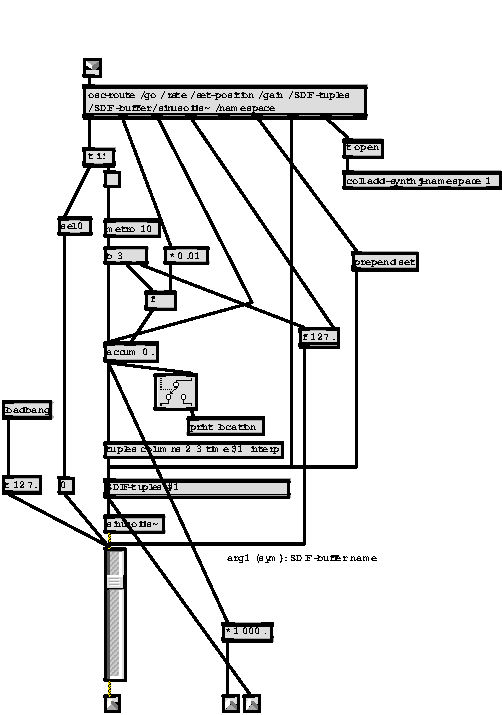
\includegraphics[width=\textwidth]{img-1-eps-converted-to-crop.pdf} 
\caption{A Max/MSP patch that performs additive synthesis in real-time using Sinusoidal Track data stored in an SDIF-buffer. Everything the patch does is accessible through a single inlet and is described by the list of OSC messages that the patch understands.}
\label{Wright:img-1}       % Give a unique label
\end{figure}

In the \textit{Tgarden} project \cite{Wei:2003}, wireless accelerometers are sensed by a Linux machine and mapped via OSC to control sound and video synthesis in Max/MSP, SuperCollider, and NATO.

\section{OSC Pedagogy}

University courses teaching OSC include the following:

\begin{itemize}
	\item Iowa State Music 448 (``Computer Music Synthesis'')
	\item Princeton COS436 (``Human Computer Interface Technology'')
	\item Stanford Music 250a (``HCI Seminar'')
	\item UC Berkeley Music 158 (``Musical Applications of Computers and Related
Technologies'') and 209 (``Advanced Topics in Computer Music'') and CNMAT's
summer Max/MSP Night School.
	\item UC Santa Barbara Music 106 (``Interactive Electronic Performance and Synthesizer
Design Using Max/MSP'')
\end{itemize}

\section{Benefits of Organizing Real-Time Music Software with OSC}

This section describes some programming techniques that make use of OSC as the
primary organizational scheme for building real-time performance instruments. 
Although our examples concentrate on the Max/MSP programming environment, the
described techniques can be generalized to other platforms and aim in general to
improve modularity and interconnectivity of software components.

\subsection{A Module's OSC Namespace Is Its Entire Functionality}

We propose a style of programming in which the entire functionality of each
software module is addressable through OSC messages. Advantages of this style
include the following:

\begin{enumerate}
	\item The OSC namespace for each module explicitly names all of that module's
features.  This can enable software to be self-documenting and transparent in its
functionality.
	\item The entire functionality of each module is accessible via a single control
mechanism: incoming OSC messages.  In graphical languages such as Max/MSP and Pd,
this allows even the most complex objects to have a single control inlet,
reducing the clutter and confusion of connecting to multiple inlets (Figure~\ref{Wright:img-1}).
As a module's functionality grows, no structural changes (such as adding more
inlets) are required; the programmer simply expands the module's OSC namespace
	\item If the components of a complex system already communicate among themselves
exclusively with OSC messages, then it becomes very easy to move some of the
components to other computers to form a distributed local area network system.
	\item Certain OSC messages can be standardized
across different modules.  For example, the message \texttt{/gain} with a floating
point argument can be used in many different synthesis and processing components
to change gain; the message ``/namespace'' can trigger any module to display its
OSC namespace; the message ``/go'' followed by the argument 1 or 0 can be used to
turn on and off the processing in the module; and the message ``/init'' can
initialize a module.
\end{enumerate}



\begin{figure}[t]
\centering
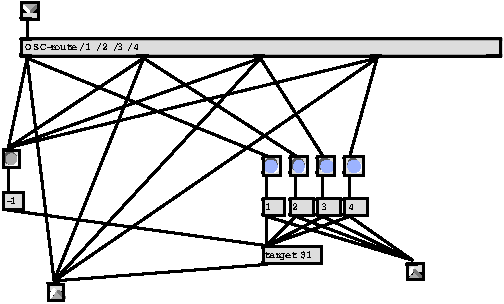
\includegraphics[width=\textwidth]{img-5-eps-converted-to-crop.pdf}
\caption{A Max/MSP patch that routes OSC messages starting with the desired voice number to that voice of a \texttt{poly~} object (which uses the \texttt{target} message to address specific voices). The patch was created with Max/MSP's scripting mechanism and could have been made with any number of voices.}
\label{Wright:img-5}       % Give a unique label
\end{figure}


By sending the ``/namespace'' message to the patch in Figure~\ref{Wright:img-1} the user is
presented with this list of OSC messages and can quickly learn how to control the
patch:

\begin{enumerate}
\item /go \_int\_ turn processing on and off;
\item /rate \_float\_ play rate;
\item /set-position \_float\_ between 0 and 1 sets position in buffer from start to;
\item /gain \_float\_ sets gain;
\item /SDIF-tuples \_anything\_ talks to SDIF-tuples;
\item /SDIF-buffer \_symbol\_ sets SDIF-buffer for playback;
\item /sinusoids\textasciitilde{} \_anything\_ talks to sinusoids\textasciitilde{};
\item /namespace \_bang\_ opens this collection;
\end{enumerate}

\subsection{Storing and Recalling Global Snapshots of Complex Software
Components with OSC}

In developing complex software instruments that perform many processes with many
possible arrangements of parameters, the task of storing and retrieving complete
snapshots of the system's state can be quite challenging.  We propose a system of
performing this storage and recalling that is based entirely on the usage of OSC
messages as the communication scheme between the instrument's snapshot mechanism
and its constituent modular components.


\begin{figure}[t]
\centering
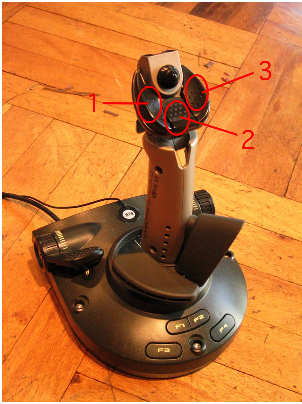
\includegraphics[width=58mm]{img-6-eps-converted-to-crop.pdf}
\caption{The Saitek Cyborg 3D joystick has 13 buttons and 4 continuous controllers. The three buttons on the top, labeled 1 to 3, can be used to route the continuous controller values to different destinations.}
\label{Wright:img-6}       % Give a unique label
\end{figure}



Once an instrument comprised of a set
of components---all of whose functionality is addressable with OSC messages---is
developed, it is possible to store and recall global settings of the entire
system by collecting and dispensing OSC messages from and to the individual
components.  We propose a model where each module keeps track of its current
state by remembering what OSC messages have been sent to it most recently.  Note
that since the OSC name for each function of the module is unique, this can be
achieved by using the OSC message as an index whose value is replaced each time a
new value is received.  In order to collect a snapshot, we query each component
for its current state.  Each component answers the query in the form of a list of
OSC message that will bring it back to its current state if sent to it at a later
time.  OSC messages from each component are then collected and stored in one
central location.  In order to recall a stored global snapshot of the system, one
simply has to send out the list of OSC messages that each component submitted
earlier.

This method was successfully employed in developing Ron Smith's work for
orchestra and live electronics titled \textit{Constellation} \cite{Madden:2001}, as well as the
collaborative dance piece of Carol Murota, Edmund Campion and Ali Momeni entitled
\textit{Persistent Vision} \cite{Campion:2002}, a work for 16 dancers and live interactive sound
installation.

\subsection{Managing Polyphony With OSC}

Many of the platforms for developing specialized real-time audio/video software
include some tools for building polyphony, e.g., Max/MSP's
\textit{poly\textasciitilde{}} object and Pd's \textit{nqpoly\textasciitilde{}}
object.  By using a simple abstraction that routes OSC messages to specific
voices of a polyphonic component (Figure~\ref{Wright:img-5}), OSC's pattern-matching features can
be used to address specific voices or sets of voices with great ease.

\subsection{Dynamic Routing of Controller Data with OSC}

We continue to advocate the use of OSC as the bridge between input data streams
from gestural controllers and signal processing engines. This style of
programming involves describing a complete OSC namespace for all output streams
from a controller \cite{Wright:2001}.  Intermediary patches dynamically map the control data to
the OSC namespace for a specific signal processing engine.  This allows the
performer to change instruments by switching from one intermediary-mapping-patch
to another, thereby directing his controller's OSC output to a different signal
processing module.

In the past year, we have further developed our implementations of this approach
to gesture mapping for a number of controllers including the Buchla Thunder,
Wacom drawing tablets (via a new interface using Cycling 74's Jitter), and the
game controller Cyborg 3D made by Saitek.

Finally, we promote the use of OSC for designing controller data streams that
are \textit{modal}.  For example, the Saitek Cyborg 3D joystick provides an
extremely flexible controller due to the number of buttons it has accessible to
the performer in conjunction with its 4 continuous controllers (Figure~\ref{Wright:img-6}).

It
is often desirable to control a number of processes with one controller, for
instance multiple voices of a polyphonic engine.  In the case of the Cyborg 3D,
OSC messages in the form of `/button-number/continuous-controller value' can be
constructed that will render the continuous contoller values \textit{modally}
addressable to different voices.  For example, holding down button 1 and moving
the joystick up and down would produce messages like, `/1/vertical value,' headed
to the first voice of our processing engine.  Holding down buttons 2 and 3 while
moving the vertical axis of the controller would produce both `/2/vertical value'
and /3/vertical value' messages, thereby controlling the second and third voices
of the processing engine.  A similar technique can be applied to any combination
of held buttons and manipulated continuous controllers to effectively turn the 4
available continuous controllers into a much larger number of control data
sources.

\section{Future of OSC}

Here are some ideas for the future of OSC. Obviously, all implementations of OSC should be completed and made consistent, able to both send and receive the full OSC spec including type tags, bundles, time tags, etc.  Full use of time tags requires solving the time synchronization problem; experiments must be done to see if NTP and SNTP will be adequate.

There is no reason that OSC should be so tied to UDP; more systems should support OSC via TCP, especially in situations where guaranteed delivery is more important than low latency.

OSC's query system is still more or less in an experimental stage; the community should standardize the syntax and semantics of a collection of useful queries.

Of course we would like to see more systems using OSC.  On the day this paper was submitted we heard that Carlos Agon had completed an initial implementation of OSC in both OpenMusic \cite{Agon:1999} and Macintosh Common Lisp. The jMax \cite{Dechelle:1999} team is also planning to implement OSC.

The translation between OSC and XML used by \textit{flosc} could be generally useful to the OSC community; we would like to see it become standardized.

\begin{acknowledgement}
Amar Chaudhary, John  ffitch, Guenter Geiger, Camille Goudeseune, Peter Kassakian, Stefan Kersten, James McCartney, Marcelo Wanderley, David Wessel.
\end{acknowledgement}


\section*{Open Sound Control: Some Context and Reflections on Thirteen Years' Advances}
\paragraph{Matthew Wright}

OSC is a widely used encoding in NIME projects and this paper (the 4th on OSC) provides practitioners with a solid introduction on what OSC is and how it they might use it. Although today we distinguish the terms ``encoding'' and ``protocol'' and tend to be more specific when talking about ``client'' and ``server,'' OSC essentially has not changed since this paper.  Receiving a message, modeled here as ``directing'' a ``kind of message'' and its ``arguments'' to ``entities'' within the receiver, can now be thought of as parallel assignment or writing to a key/value store such as a ``record,'' ``dictionary,'' ``associative array,'' or `` property list,'' but the underlying interoperable machinery remains substantially identical.  Today's wealth of OSC APIs and libraries for most active programming languages (including the 38 ``programming language libraries'' on opensoundcontrol.org) allows most users to ignore the details of the encoding.

This was the first OSC paper to describe type tags, one of the only new features since the original 1997 ICMC paper. Credit belongs to James McCartney, who needed to support situations where the sender did not know in advance what types the receiver expected for each message, or where type polymorphism (same message name, different argument types) was desired. Just as CNMAT had unilaterally defined and implemented OSC, McCartney unilaterally defined and implemented OSC type tags (originally optional, hence the funny comma character), which CNMAT later adopted and are now universal.

Today OSC-encoded packets are embedded in many kinds of data streams and transported among devices with different wired and wireless protocols, including SLIP via USB serial or ``TTL'' serial; TCP via web-, UNIX, or Windows sockets; and most often UDP packets via TCP/IP based LANs and WANs. 

OSC use preceded that of the popular XML and JSON encodings, which both have simpler representations for hierachical data than OSC's anonymous recursive subbundles (which are rarely implemented, tested, or used).  OSC now supports bundles as message arguments.

This paper continued our tradition of talking about a query system that didn't really exist;  today there are several incompatible query systems none widely implemented.  The paper's optimism that ``obviously'' all implementations would eventually support every feature of OSC has given way to accepting the fact that there will always be incomplete implementations.

OSC has traveled into many different development communities who use it in innovative ways not envisaged by its inventors. Although in 2003 we believed we were aware of almost all OSC use, the full history and extent of its cultural uptake is still to be carefully chronicled.  Although the existence of the OSC Kit may have helped adoption of OSC, to our knowledge nobody actually fully used it as designed. Some implementations used portions of it (e.g., pattern matching) but most reimplemented OSC until the existence of other libraries such as oscpack and liblo. On the other hand, sendOSC and dumpOSC are still indispensable, confirming whether valid messages are sent and their contents (or the specific problem if invalid), and helping troubleshoot networks, firewalls, address space mismatches, faulty arguments, etc.

OSC has also traveled to many creative communities outside of computer music.  Within the domains of virtual and augmented reality (Unity, Unreal Engine), staged dramatic works with complex media-design (Processing, OpenFrameworks, D3, Millumin, Madmapper, TouchDesigner), modeling and fabrication (Rhino Grasshopper with gHowl), physical computing and internet of things applications (software: ROS, oscuino, Maxuino; hardware: Particle SparkCore, ESP8266) many practitioners are adapting OSC for their needs in communicating among several processes, platforms, or locations.  

We offer this broad taxonomy of current use patterns:

\begin{enumerate}
	\item Client/server: e.g., communications between computers optimized for user interaction (e.g. Apple Macintosh) and machines optimized for computing performance (e.g. SGI O2), Meyer/LCS spatial audio and show control
	\item Inter-Process communication, e.g., between Max and synthesis ``servers'' on the same machine, Supercollider, OpenSound World...
	\item Inter-Media synchronization and communication, e.g. between Unity as a real-time visual virtual reality and max as a synthesizer for responsive environmental sound
	\item Synchronization and automation, netjamming, ICMC paper from IRCAM
	\item Transcoding and wrapping (as described in Section 5.4), e.g., TUIO for multitouch, DMX lighting control, many wrappers in CNMAT's MMJ Depot and o.io.
	\item Native encoding for input and output devices (MIDI alternative), e.g., Monome, OSC for Arduino, many phone and tablet apps.  (We note that all of the commercial hardware projects listed in Section 2.6 are now gone, but many others have taken their place)
	\item Extension language (o dot, gdif, spatdif)
	\item dynamic programming hooks (OSW, 
\end{enumerate}
 
Regarding education, though in 2003 institutions teaching OSC were noteworthy, today one would expect OSC in any computer music or interactive digital arts program and especially in any hands-on NIME course.


\section*{Expert Commentary: OpenSound Control: State of the Art 2003}


\paragraph{Roger B. Dannenberg}


OpenSound Control (OSC) has become a standard building block for not only music systems but any number of interactive art installations, virtual reality systems, and other systems needing distributed control and communication. OSC follows a long history of protocols including MIDI for music, ZIPI, intended to extend and replace MIDI, CORBA and DCE, middleware for distributed computing. A series of protocols for the Web followed earlier developments, resulting in HTTP, SOAP, REST, and certainly more will come. With all these distributed systems protocols, it is surprising that OSC has gained so much traction. Why OSC?

John Huntington \cite{Huntington:2008} describes some ``common attributes of successful standards,''including ``Successful standards are pulled into existence by the market; they are not pushed. They fill a clear commercial demand in the market, especially one driven by users.'' One could argue that OSC greatly simplified existing standards and better met the requirements of interactive music programs. However, even ZIPI was said to have an ``unusual addressing scheme which required substantial increase in complexity,'' \cite{Wikipedia:2014} and OSC's addressing scheme is even more complex. When announced, many complained that the pattern-matching features in OSC and the URL-like addresses would be too slow and difficult to implement. On the other hand, OSC arguably was and still is too simple. OSC was modified to include datatype information and is still considered to have problems with queries, discovery, timestamps, and the use of different transports. Whatever the reasons, OSC has been wildly successful, especially as an open technology with academic origins.

One explanation for OSC's popularity could be that it lowers the barriers to interfacing with Max/MSP and Pd \cite{Puckette:2002}, two very popular visual programming systems used by musicians and artists. Without OSC, one can extend Max/MSP or Pd by writing ``external'' objects in C, but this requires a rather detailed knowledge of internal program structures and interfaces. Once OSC ``objects'' were created for Max/MSP and Pd, one could extend these programs through OSC. For example, one can now build a sensor that sends data through very simple network packets. Using OSC with Max/MSP and Pd solves both the connection problem (just use Ethernet or WIFI) and the interface problem (forming and sending simple network packets is simpler than developing ``externals''). The inter-operability, modularity, and distributed processing support resulting from a network-based protocol are all added attractions, but could it be that the desire to connect to Max and Pd drove widespread adoption of OSC?

What is next? When OSC was announced, the fastest personal computers were comparable to today's smartphones. Now that even low-cost embedded processors used for sensors are quite capable of running sophisticated software, one can imagine much more powerful protocols being deployed as ``standards'' in the worlds of interactive art and music. But going back to systems like CORBA seems unlikely to catch hold. A lesson we can take from OSC and the Web is that, while highly optimized binary protocols may be attractive for performance, the flexibility of symbolic addresses and late or dynamic binding is more important to most users. I can imagine the next generation of interprocess control being built upon bi-directional network connections where every node runs an active server to offer named services (as opposed to IP addresses and port numbers most often used with OSC), peer-to-peer connections, automatic routing, clock synchronization \cite{Brandt:1999}, web interfaces for performance monitoring and testing, and many other services. Clients might construct URL-like requests that specify a destination by name (``audio-mixer'') to be routed automatically to the node providing that resource. Of course, this would represent a big step up in complexity from OSC, but it might make things simpler for end users.

Whatever happens in the future, OSC has established itself as a versatile standard for inter-process communication, enabling countless systems to be constructed in a modular and flexible way. This paper, ``OpenSound Control: State of the Art 2003,'' gives an excellent overview of OSC, the designer's intentions, and how applications use OSC. More than 10 years later, the article is still an excellent way to become acquainted with OpenSound Control.
